%%%%%%%%%%%%%%%%%%%%%%%%%%%%%%%%%%%%%%%%%
% FRI Data Science_report LaTeX Template
% Version 1.0 (28/1/2020)
% 
% Jure Demšar (jure.demsar@fri.uni-lj.si)
%
% Based on MicromouseSymp article template by:
% Mathias Legrand (legrand.mathias@gmail.com) 
% With extensive modifications by:
% Antonio Valente (antonio.luis.valente@gmail.com)
%
% License:
% CC BY-NC-SA 3.0 (http://creativecommons.org/licenses/by-nc-sa/3.0/)
%
%%%%%%%%%%%%%%%%%%%%%%%%%%%%%%%%%%%%%%%%%


%----------------------------------------------------------------------------------------
%	PACKAGES AND OTHER DOCUMENT CONFIGURATIONS
%----------------------------------------------------------------------------------------
\documentclass[fleqn,moreauthors,10pt]{ds_report}
\usepackage[english]{babel}

\graphicspath{{fig/}}
\usepackage{graphicx}  % Add this to your preamble if it's not already there




%----------------------------------------------------------------------------------------
%	ARTICLE INFORMATION
%----------------------------------------------------------------------------------------

% Header
\JournalInfo{FRI Natural language processing course 2025}

% Interim or final report
\Archive{Project report} 
%\Archive{Final report} 

% Article title
\PaperTitle{Automatic Generation of Slovenian Traffic News for RTV Slovenija} 

% Authors (student competitors) and their info
\Authors{Filip Turk and Tschimy Aliage Obenga}

% Advisors
\affiliation{\textit{Advisors: Slavko Žitnik}}

% Keywords
\Keywords{Generating traffic reports, Large Language Models, NLP, Prompt Engineering, Fine-tuning, Slovenian traffic news, Automated text generation}

\newcommand{\keywordname}{Keywords}


%----------------------------------------------------------------------------------------
%	ABSTRACT
%----------------------------------------------------------------------------------------

\Abstract{
This paper presents a data-centric methodology for automating the generation of Slovenian traffic news for RTV Slovenija. Recognizing that real-world data is often inconsistent, we first developed a robust data processing pipeline to create a high-quality, aligned dataset from noisy source materials provided by Promet.si. This pipeline employs semantic similarity matching to overcome temporal discrepancies and regular expressions to structure unstructured text into a clean JSON format. Using this curated dataset, we compared two approaches: (1) parameter-efficient fine-tuning (PEFT) of a native Slovenian model (GaMS-9B) and (2) a multi-step prompt engineering strategy with a powerful general-purpose model (Google's Gemini-2.5-flash). Our comprehensive evaluation, which includes both automated metrics and human assessment, demonstrates that the prompt-engineered Gemini pipeline significantly outperforms the fine-tuned model. It successfully produces factually accurate, stylistically compliant, and broadcast-ready reports, underscoring that for complex, real-world NLP tasks, a sophisticated data preprocessing and advanced prompting strategy can be more effective than fine-tuning on inherently inconsistent data.
}


%----------------------------------------------------------------------------------------

\begin{document}

% Makes all text pages the same height
\flushbottom 

% Print the title and abstract box
\maketitle 

% Removes page numbering from the first page
\thispagestyle{empty} 

%----------------------------------------------------------------------------------------
%	ARTICLE CONTENTS
%----------------------------------------------------------------------------------------

\section*{1. Introduction}
The dissemination of timely and accurate traffic information is a critical public service. At RTV Slovenija, this task relies on a manual workflow where students monitor the Promet.si portal, interpret raw traffic data, and compose broadcast announcements every 30 minutes. This process is labor-intensive and prone to inconsistencies in style, tone, and information priority, making it an ideal candidate for automation using Large Language Models (LLMs).

However, automating such a task is non-trivial. The primary challenge lies not just in generating fluent text, but in navigating the inherent noise and inconsistency of real-world data sources. The "ground truth" itself, represented by past human-written reports, often suffers from variability due to subjective human judgment. A model trained naively on such data risks learning these inconsistencies, leading to unreliable or "hallucinated" outputs.

Anticipating this challenge, we adopted a data-centric approach. This paper details our methodology, which prioritizes the creation of a high-quality, structured dataset as a foundation for reliable text generation. We present the following key contributions:
\begin{enumerate}
    \item A \textbf{semantic data alignment pipeline} that processes raw traffic reports, matches them with corresponding official announcements using cosine similarity, and structures them into a clean categorized JSON format (Appendix 1).
    \item A comparative analysis of two distinct strategies: \textbf{fine-tuning} a specialized Slovenian model (GaMS-9B) and employing a \textbf{multi-step prompt engineering} approach with a general-purpose model (Gemini-2.5-Flash).
    \item A comprehensive evaluation demonstrating that the combination of a high-quality dataset and advanced prompting yields superior, broadcast-ready results, providing a robust blueprint for real-world NLP applications.
\end{enumerate}


\section*{2. Literature Review and Related Work}

\subsection*{Automated News Generation Systems}
Recent developments in automated journalism have demonstrated the viability of AI-driven content generation across various domains. Notable implementations include Google's automated sports reporting systems and Reuters' financial news generators, which leverage structured data to produce coherent narratives. These systems typically employ template-based approaches combined with natural language generation techniques.

\subsection*{Large Language Models for Low-Resource Languages}
The advancement of multilingual LLMs has opened new possibilities for automated text generation in languages with limited computational resources. The GaMS (Generative AI Models for Slovenian) project represents a significant contribution to Slovenian NLP, providing pre-trained models specifically optimized for Slovenian language tasks. These models demonstrate superior performance compared to general-purpose multilingual models when processing Slovenian text.

\subsection*{Parameter-Efficient Fine-Tuning}
Low-Rank Adaptation (LoRA) has emerged as a prominent technique for efficient model adaptation, enabling fine-tuning of large models with minimal computational resources. This approach has proven particularly effective for domain-specific applications, allowing practitioners to adapt pre-trained models to specialized tasks without extensive hardware requirements.

\section*{3. Initial Experiments and the Data Bottleneck}
Before developing our full data processing pipeline, we first conducted a series of baseline experiments to assess the viability of using off-the-shelf models with minimally processed data. For this initial phase, we created a dataset by performing a simple temporal match: pairing each RTV announcement with the most recent Promet.si source report that preceded it.

\subsection*{3.1. Zero-Shot and Few-Shot Prompting on GaMS}
Our first attempt involved prompt engineering with the GaMS-2B model. We designed comprehensive one-shot and few-shot prompts that included diverse examples of traffic scenarios and explicit instructions on adhering to RTV's reporting style. However, the results were consistently poor. The generated text suffered from grammatical errors, factual inaccuracies (hallucinations), and a failure to capture the correct broadcast tone. Increasing the model size to GaMS-9B yielded no significant improvements, indicating that the problem was not a lack of model capacity.

\subsection*{3.2. Fine-tuning on Temporally Matched Data}
Given the failure of prompting, we hypothesized that fine-tuning would allow the model to learn the specific nuances of the task. We proceeded to fine-tune the GaMS-9B-Instruct model using LoRA on this temporally-matched, un-curated dataset. The technical setup involved 4-bit quantization via BitsAndBytes and training on the ARNES HPC cluster, with the implementation managed by the TRL library's SFTTrainer.

While the fine-tuned model showed a slight improvement in semantic relevance (as measured by BERTScore), the qualitative results remained unacceptable for real-world use. The model continued to hallucinate information, and the lexical and structural similarity to the ground truth was negligible, as reflected in near-zero BLEU and ROUGE scores.

\subsection*{3.3. Identifying the Root Cause}
The consistent failure of both prompting and fine-tuning led to a critical conclusion: the bottleneck was not the model or the training methodology, but the data itself. A manual analysis of our temporally-matched dataset revealed severe inconsistencies. The human-written RTV announcements often omitted crucial information present in the source, rearranged event priority without a discernible pattern, and varied significantly in style. By training on this noisy, one-to-one temporal mapping, we were inadvertently teaching the model to replicate this randomness, which manifested as poor performance and hallucination. This insight necessitated a complete pivot in our approach, shifting our focus from model-centric solutions to a data-centric one, which is detailed in the following section.

\section*{3. Data refinement}

\subsection*{Data Processing and Semantic Alignment}
The quality of any supervised model is contingent on the quality of its training data. Our analysis revealed significant discrepancies between the raw input data from Promet.si and the final RTV announcements. A simple time-based mapping was insufficient, as reports were often delayed, and the information included was a subjective subset of what was available. To address this, we designed a multi-stage data processing pipeline.



\subsection*{3.1. Semantic Matching}
Instead of relying on rigid timestamps, we implemented a semantic matching process. For each target RTV announcement, we created a candidate pool of source reports from Promet.si within a flexible $\pm$60-minute window. We then used a pre-trained sentence-transformer model to compute the cosine similarity between the vector embeddings of the target announcement and each candidate report. The candidate with the highest similarity score was selected as the most contextually relevant input, ensuring a strong semantic link between our input-output pairs. This process yielded an initial dataset of 22,112 pairs with a near-gaussian similarity distribution peaking at approximately 0.7.

\subsection*{3.2. Data Structuring and Cleaning}
The raw source data was provided as dataframe of categorized information regarding  the current state of traffic including semi-structured HTML parts. We used a series of regular expressions to parse this data, categorizing information into a standardized JSON object. This object contains predefined keys such as \texttt{"Nesreče"} (Accidents), \texttt{"Zastoji"} (Congestion), and \texttt{"Dela na cesti"} (Roadworks), etc, creating a fully structured and categorized input.

Furthermore, we performed two cleaning steps. First, we identified and removed recurring boilerplate phrases (e.g., "Vir: DARS," "Več informacij na...") that were present in the source but never in the final RTV report. Second, we normalized all temporal expressions. Specific dates were converted into relative terms like "jutri, pojutrišnjem, včeraj, danes" (toomorow, in two days, yesterday, today) based on the report's timestamp, providing unambiguous temporal context to the model.

\subsection*{3.3. Quality Filtering}
To ensure the highest data quality for our experiments, we filtered the dataset by removing all pairs with a cosine similarity score below 0.7. This step was crucial to eliminate instances where the semantic link between the source and target was weak, thereby preventing the model from being trained on noisy or mismatched examples. The final, curated dataset formed the foundation for our prompting experiments.

\begin{figure}[ht]\centering
    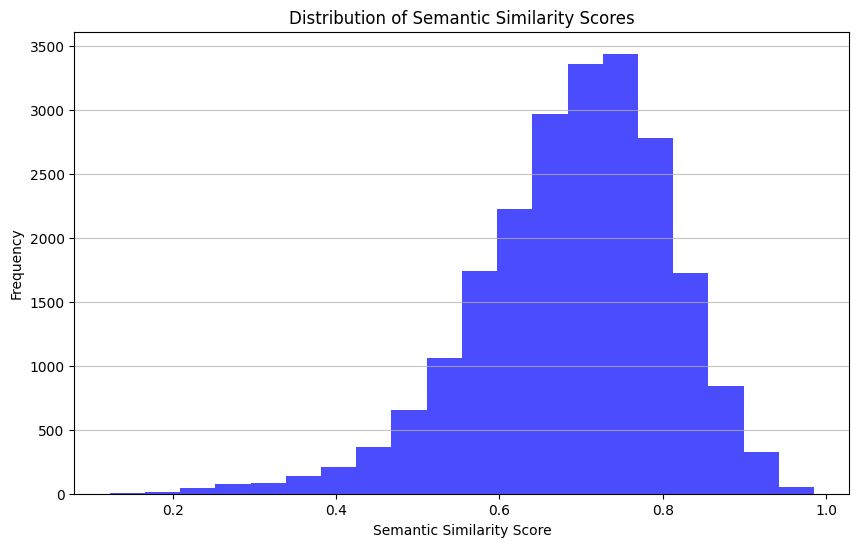
\includegraphics[width=\linewidth]{fig/SimilarityScore_01.png}
    \caption{\textbf{Semantic similarity} This plot compares the semantic similarity scores (cosine similarity) between input information and human generated traffic reports.}
    \label{fig:similarity-bert-single}
\end{figure}

\section*{4. Experimental Methodology}
OHaving established a high-quality, structured, and semantically aligned dataset, we designed a new set of experiments to compare two distinct generative strategies. The first strategy involved fine-tuning the specialized GaMS-9B model again, using the refined data, while the second utilized a multi-step prompting pipeline with the general-purpose Gemini (Flash-2.5) model. This direct comparison was designed to identify the most robust path to generating high-quality traffic news.

\subsection*{4.1. Method A: Fine-tuning GaMS-9B on Curated Data}
To provide a fair comparison and test our hypothesis that data quality was the primary bottleneck, we revisited our fine-tuning approach. We performed a new fine-tuning run of the GaMS-9B-Instruct model using LoRA. However, this time we used our new high-quality dataset, filtered to include only pairs with a cosine similarity score above 0.7. The technical setup remained consistent with our initial experiments to isolate the impact of the data quality. 

\subsection*{4.2. Method B: Two-Step Prompting with Gemini 2.5 Flash}
Our second approach leveraged a general-purpose model, Google's Gemini 2.5 Flash, with a prompting strategy that mirrors a human workflow of drafting and refining. This method breaks the complex task into two sequential steps:

\begin{enumerate}
\item \textbf{Generation Prompt:} The model first receives the structured JSON data along with an input message created from the JSON data. The initial prompt instructs it to synthesize this information into a single, coherent, and descriptive paragraph. The goal of this step is pure information synthesis—transforming structured data into fluent natural language without heavy initial stylistic constraints.

\item \textbf{Refinement Prompt:} The output from the generation step is immediately fed back into the model with a second, more specific prompt. This "refiner" prompt acts as an editor, instructing the model to:
\begin{itemize}
    \item \textbf{Reorder events} according to RTV's implicit priority (e.g., major accidents and highway congestion before minor roadworks).
    \item \textbf{Filter for relevance}, removing information that is often omitted in human-written reports.
    \item \textbf{Ensure a professional, telegrafic tone} by removing conversational fillers and greetings (e.g., "Srečno vožnjo," "Pozor vozniki").
    \item \textbf{Standardize phrasing} to match the broadcast style.
\end{itemize}

\end{enumerate}
This pipeline approach decouples the task of information synthesis from stylistic formatting, allowing for more granular control over the final output and directly addressing the issues of relevance and event ordering identified in initial tests.
\section*{5. Results and Analysis}
We evaluated both methods and the intermediate step of the Gemini pipeline using a combination of automated metrics and human assessment. For the human evaluation, a sample of generated reports was rated on a scale of 1 to 5. The evaluation was based on six key criteria tailored to the requirements of broadcast-ready traffic news:

\begin{itemize}
    \item \textbf{Truthfulness:} Does the generated report contain only information present in the source JSON? A low score indicates hallucination.
    \item \textbf{Relevance:} Does the report prioritize important events and omit minor details or events, mimicking a human editor's judgment?
    \item \textbf{Grammar:} Is the text grammatically correct in Slovenian?
    \item \textbf{Readability:} Is the report fluent, concise, and easy to understand when read aloud?
    \item \textbf{Order of Events:} Does the report follow the implicit RTV hierarchy (e.g., major highways and accidents before minor roadworks)?
    \item \textbf{Timeliness:} Does the model correctly use relative temporal expressions like "danes" or "jutri" instead of raw dates when applicable?
\end{itemize}

\subsection*{5.1. Performance of the Fine-tuned GaMS-9B-Instruct Model}
The evaluation metrics reveal the significant limitations of the fine-tuned GaMS-9B-Instruct model. Despite being trained on the refined dataset, its outputs continued to exhibit poor lexical and structural similarity to the reference texts, resulting in extremely low BLEU scores. Qualitative analysis confirmed these shortcomings: the model was prone to factual hallucinations, often inventing information not present in the source data. Furthermore, it occasionally failed to correctly parse the input, leaking technical artifacts such as JSON keys into the generated text or simply just repeating the input information verbatim. While its grammatical structure was generally coherent, it was qualitatively inferior to the Gemini-generated outputs. The fact that performance did not substantively improve with the refined dataset strongly indicates that the model itself, rather than the data, is the primary bottleneck. We, therefore, conclude that it is not a suitable candidate for this specific, complex generation task.

\subsection*{5.2. Performance of the Two-Step Gemini Pipeline}
In stark contrast, the two-step Gemini pipeline proved highly effective, demonstrating strong performance that was significantly enhanced by the refinement step.

The initial generation step produced grammatically correct and highly readable text, achieving a strong baseline in both automated metrics and human scores for Grammar (4.60) and Readability (4.80). However, human evaluation confirmed its primary weaknesses: a tendency to include non-essential information (Relevance: 2.53) and a suboptimal ordering of events (Order of Events: 4.07).

The second, "refiner" step was specifically designed to address these shortcomings and was exceptionally successful. The final output saw marked improvements in relevance and event ordering, achieving perfect or near-perfect scores across all human-judged criteria, including a perfect 5.00 for Truthfulness. This qualitative improvement was mirrored in the automated metrics, where achieved the highest BERTScore (F1: 0.8711) and the best BLEU scores, confirming a close alignment with the style and structure of the reference reports.

Qualitatively, the final reports from the two-step Gemini pipeline are consistently truthful and concise, adhering to the required telegrafic tone. While the pipeline successfully filters many irrelevant details, a deeper analysis reveals a fundamental limitation rooted in the data itself: a discrepancy often exists between the information available in the Promet.si source data and the final human-written RTV reports. In some instances, the ground truth contains information not present in our structured input.

Our pipeline, by design, cannot report on information it is not given. Its greatest strength, however, is its factual integrity. Unlike the GaMS model, it does not hallucinate to fill these data gaps, instead generating a coherent and accurate report based strictly on the provided input. Therefore, the model performs exceptionally well within the constraints of the available data, producing outputs that are highly reliable and suitable for direct broadcast with minimal human oversight. This establishes a robust baseline, with further improvements being contingent on access to a more comprehensive data source.

\section*{6. Conclusion and Future Work}
This project successfully demonstrates a robust, data-centric approach to automating the generation of specialized news content. Our findings reveal a critical insight for real-world NLP applications: when faced with inherently inconsistent or noisy ground-truth data, a sophisticated data processing pipeline combined with advanced prompt engineering on a powerful base model can be a more effective strategy than fine-tuning a under-resourced specialized model. Even with a curated dataset, the fine-tuned GaMS-9B model failed to produce usable results, whereas Gemini pipeline produced high-quality, broadcast-ready Slovenian traffic reports that meet the stringent requirements of RTV Slovenija.
For future work, several avenues are promising. First, using our high-quality, curated dataset to now fine-tune a powerful model like Gemini could potentially combine the strengths of both approaches, yielding even better results by embedding the stylistic nuances directly into the model's weights. Second, a closer collaboration with RTV to further standardize their reporting guidelines would create an even cleaner ground truth, simplifying the data pipeline and improving model reliability. Finally, the development of a real-time deployment pipeline with a human-in-the-loop interface would allow for continuous monitoring, correction, and collection of high-quality data for ongoing model improvement.

%----------------------------------------------------------------------------------------
%	REFERENCE LIST
%----------------------------------------------------------------------------------------

\begin{thebibliography}{9}

\bibitem{huggingface}
Wolf, T., et al. (2020).
\textit{Transformers: State-of-the-Art Natural Language Processing}.
HuggingFace.
\url{https://huggingface.co/docs}

\bibitem{lora}
Hu, E. J., et al. (2021).
\textit{LoRA: Low-Rank Adaptation of Large Language Models}.
arXiv preprint arXiv:2106.09685.
\url{https://arxiv.org/abs/2106.09685}

\bibitem{trl}
von Werra, L., et al. (2023).
\textit{TRL: Transformer Reinforcement Learning}.
HuggingFace.
\url{https://huggingface.co/docs/trl}

\bibitem{gams}
Ulčar, M., et al. (2023).
\textit{GaMS: Generative AI Models for Slovenian}.
CJVT.
\url{https://huggingface.co/cjvt/gams-9b}

\bibitem{datasets}
Lhoest, Q., et al. (2021).
\textit{Datasets: A Community Library for Natural Language Processing}.
HuggingFace.
\url{https://huggingface.co/docs/datasets}

\bibitem{rtv}
RTV Slovenija. (2024).
\textit{Traffic Report Guidelines and Standards}.
Internal documentation.

\end{thebibliography}

%----------------------------------------------------------------------------------------
%	APPENDIX
%----------------------------------------------------------------------------------------



% Use the table* environment to make the table span both columns on the page.
% The [t] specifier places it at the top of the next page where it fits.
\begin{table*}[t] 
\centering
\caption{Combined Automated and Human Evaluation Metrics. }
\label{tab:combined_results_appendix}
\begin{tabular}{lccc}
\toprule
\textbf{Metric} & \textbf{Gemini (Pipe 1)} & \textbf{Gemini (Pipe 2)} & \textbf{GaMS-9B (Pipe 3)} \\ 
\midrule
% Subheading for Automated Metrics
\multicolumn{4}{l}{\textit{Automated Metrics}} \\
\quad BERTScore F1    & 0.8684                   & \textbf{0.8711}          & 0.8535 \\
\quad BLEU-1          & 0.2307                   & \textbf{0.2509}          & 0.1495 \\
\quad BLEU-2          & 0.1379                   & \textbf{0.1486}          & 0.0952 \\
\quad BLEU-3          & 0.0920                   & \textbf{0.1021}          & 0.0691 \\
\quad BLEU-4          & 0.0630                   & \textbf{0.0677}          & 0.0513 \\
\midrule
% Subheading for Human Evaluation
\multicolumn{4}{l}{\textit{Human Evaluation (Rated 1-5)}} \\
\quad Truthfulness    & 4.00 & \textbf{5.00} & 1.07 \\
\quad Relevance       & 2.53 & \textbf{2.88} & 1.07 \\
\quad Grammar         & 4.60 & \textbf{5.00} & 1.43 \\
\quad Readability     & 4.80 & \textbf{5.00} & 1.50 \\
\quad Order of Events & 4.07 & \textbf{4.88} & 1.43 \\
\quad Timeliness      & 4.60 & \textbf{5.00} & 1.64 \\ 
\bottomrule
\end{tabular}
\end{table*}

% --- TABLE 1 ---
\end{document}% --- TABLE 1 ---
\end{document}